\documentclass{book}
\usepackage{mathtools}
\usepackage{tikz}
\usetikzlibrary{positioning}

\usepackage{amsthm}
\usepackage{amsmath}
\usepackage{amssymb}

\newtheorem{defn}[equation]{Definition}
\newtheorem{coro}[equation]{Corollary}
\newtheorem{prop}[equation]{Proposition}
\renewenvironment{proof}{\emph{Proof}}{\qed}


\begin{document}

\section{Foreword}
In transitioning to more advanced classes, a physics student will find their familiar mathematical tools are inadequate to describe certain physical phenomena. The methods of traditional vector calculus in three dimensions, though very useful in electromagnetism and classical mechanics, are not always usable in higher dimensions, such as those used in general relativity and Hamiltonian mechanics. For that, we need differential geometry. When trying to learn a subject in mathematics, however, you tend to find books written for mathematicians, in a language that mathematicians are familiar with. As such, they are filled with long, obtuse definitions and prose that, while mathematically very precise, isn't exactly light reading, and can even be overkill for a proper physical understanding. 

What follows is a purely physical treatment of differential geometry used in physics. While it is less mathematically rigorous than a typical textbook, the hope is that the reader will be able to gain a geometric intuition for the math they use, so that the math isn't simply a black box beyond understanding, and that further study in the subject will be aided by a solid grounding here. The focus is always on readability, applicability, and physicality, so pictures are prevalent (\textbf{\textit{Will} be prevalent}). 




\tableofcontents




\chapter{Mathematical representations of physical objects}



\section{Physical objects and quantities}

At the heart of scientific investigation is the identifying and organizing of objects based on their properties, through measurement and experiment. This could be anything from setting a block on a scale to determine its weight to determining the species that a particular animal belongs to. For our purposes here, we will be dealing only with properties that can be described using real numbers, such as mass, temperature, velocity, etc. The identification of a particular physical property with a real number is a \textbf{quantity}.

\begin{defn}
	A \textbf{quantity} is a function $q : U \to \mathbb{R}$ that assigns a measurable value to a physical object.
\end{defn}



It's quite possible, however, that we won't be able to distinguish between two objects with only one quantity. Say, for instance, that we're talking about weather. Knowing what the temperature will be tomorrow is certainly useful, but as anyone from Florida can tell you, 80$^o$F with 95$\%$ humidity is very different than 80$^o$F with 30$\%$ humidity. In distinguishing objects, then, we will often want to define more than one quantity, to give an even more descriptive way of categorizing objects. By defining enough quantities to distinguish one case from another, but not so many such that we have redundancies, we can define a \textbf{coordinate system}.


Normally, we think of coordinate systems in the context of quantifying an object's position, in terms of its x-, y-, and z-coordinates, but this is just a specific case. Coordinate systems as discussed here are far more general, and find immediate application throughout physics. Consider, for instance, phase space. Configurations in phase space can be distinguished by position as well as by momentum, which would be our two quantities, thus giving us a coordinate system. 

\begin{defn}
	A \textbf{coordinate system} $Q$ is a collection of $n$ quantities $q^i : U \to \mathbb{R}^n$ such that there is a one-to-one relationship between the physical objects in $U$ and elements of $\mathbb{R}^n$.
\end{defn}






With coordinate systems now defined, we recognize that in many instances, two different coordinate systems function just as well to describe a certain object. Mathematically, this occurs when two sets, each with defined coordinate systems, overlap. The points that lie within this overlapping section may be described in either coordinate system. To give an example from geography, consider an atlas of the world: a collection of maps. Depending on the atlas you're looking at, certain places may show up in multiple maps. Consider Moscow, for instance. It could very well show up on a map of Asia, perhaps in a square labeled B2, while also showing up on a map of Europe, perhaps in a square labeled C8. Either way of describing Moscow's position is equally valid, and you can freely "transform" between the coordinate systems as far as Moscow is concerned. Alternatively, consider the "point" Lisbon. Lisbon will show up on a map of Europe, perhaps in square F1, but you would never find Lisbon on a map of Asia. Therefore, its position may only be described in terms of the coordinates on the map of Europe.


\begin{defn}
	Given two coordinate systems  $Q : U \to \mathbb{R}^n$ and $Q' : V \to \mathbb{R}^n$ such that $U \cap V \neq \emptyset$, we call a \textbf{coordinate transformation} the function $f = Q' \circ (Q)^{-1} : \mathbb{R}^n \to \mathbb{R}^n$.
\end{defn}



\textbf{May have to describe the meaning of the diagram, reader might not know. Or take it out}
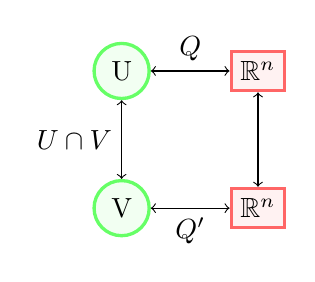
\begin{tikzpicture}
[roundnode/.style={circle, draw=green!60, fill=green!5, very thick, minimum size=7mm},
squarednode/.style={rectangle, draw=red!60, fill=red!5, very thick, minimum size=5mm},
]
\node[roundnode]	(U) {U};
\node[roundnode]	(V) [below=of U]{V};
\node[squarednode]	(realU) [right=of U] {$\mathbb{R}^n$};
\node[squarednode]	(realV) [right=of V] {$\mathbb{R}^n$};

\draw[<->] (U) -- (realU) node[midway, above] {$Q$};
\draw[<->] (U) -- (V) node[midway, left] {$U\cap V$};
\draw[<->] (V) -- (realV) node[midway, below] {$Q'$};
\draw[<->] (realU) -- (realV);
\end{tikzpicture}

Consider now a set of configurations of a system. Every one of these configurations is somehow mappable to the real numbers, with an appropriate coordinate system. However, a specified coordinate system may not be applicable to every point in the set. What we have, therefore, is a stitched-together collection of sets of configurations, each of which contains a map to the real numbers. This is a \textbf{manifold}. 

\begin{defn}
	A \textbf{manifold} is a set of physical objects $X$ such that for any $x \in X$ there exists a $U \subset X$ that contains $x$ and upon which a coordinate system $Q$ is defined.
\end{defn}


Earlier, weather was given as an example of a set possible cases of a system, with readings such as temperature and humidity allowing us to define a coordinate system. In this context, the "manifold" would be the set of possible weather configurations, with each point being a single weather report. 

The Earth is a classic example of a manifold, which allows for further discussion of the geography example. Because of the poles, every location on earth cannot be quantified with only one set of coordinates. This can be plainly seen on a typical flat map, such as a Mercator Projection. Land proportions grow the closer to a pole they are, making Greenland appear massive, and the Sahara proportionally far smaller. Furthermore, because the poles have been unraveled, in a sense, the South Pole, which ought to be a single point, is an entire line along the southern edge of the map. A proportionally accurate projection of the Earth onto a flat surface requires at least two separate maps. For instance, you could then have a map of the top hemisphere, centered at the north pole, and then of the bottom hemisphere, centered at the south pole. 



\textit{Talk about a lot of different examples, so that manifolds are clearly everyday objects}

\textbf{Insert a picture of the Mercator Projection}

\textbf{Insert pictures of "polar" projections}

Another example of a manifold would be the possible results of a blood drawing. The doctor takes your blood for analysis, the results of which are collected on a report, detailing things such as blood pressure, cholesterol levels, white blood cell count, etc. Further examples include: 

- The conditions of your car, with the dials on the dashboard being your method of reading them 

- The freight on a ship, with the bill of lading detailing amounts

- Any sort of information that can be condensed down to a series of real numbers

The plethora of examples is to show the ubiquitousness of manifolds, and that they are very familiar, everyday objects. This versatility proves their usefulness in physics, and in scientific investigation in general. 

\section{Sub-manifolds and k-surfaces}

Consider an n-dimensional manifold; that is, a manifold with n degrees of freedom. We can construct another manifold with k degrees of freedom within the original, as long as k is not greater than n. Back to the weather example, if in the original weather report we were worrying about temperature, humidity, and wind speed, we could instead hold one of the three values fixed (say, humidity), and vary the other two. The latter manifold, with humidity held constant, would be a \textbf{submanifold} of the former, where all three variables are allowed to change. The boundary of this smaller manifold occurs where the varying is stopped by one means or another. 
\textit{Define boundary up here instead of further down}


\begin{defn}
	Consider a manifold X of dimension n, and a manifold Y of dimension k, such that $k \leq n$. Y is a \textbf{submanifold} or a \textbf{k-surface} of X if any point on Y is also a point on X. 
\end{defn}

\begin{tikzpicture}
[roundnode/.style={circle, draw=green!60, fill=green!5, very thick, minimum size=7mm},
squarednode/.style={rectangle, draw=red!60, fill=red!5, very thick, minimum size=5mm},
]
\node[roundnode]	(X) {X};
\node[roundnode]	(Y) [below=of X]{Y};
\node[squarednode]	(realX) [right=of X] {$\mathbb{R}^n$};
\node[squarednode]	(realY) [right=of Y] {$\mathbb{R}^k$};

\draw[<->] (X) -- (realX) node[midway, above] {$Q$};
\draw[->] (X) -- (Y) node[midway, left] {$U\cap V$};
\draw[<->] (Y) -- (realY) node[midway, below] {$P$};
\draw[->] (realU) -- (realV);
\end{tikzpicture}

In general, we will be using the term "k-surface", instead of "submanifold." There will be many terms throughout this thesis prefaced by "k-". In general, this means that the object in question has k degrees of freedom. Such objects will be sorted based on the number of degrees of freedom that they have.  


\begin{defn}
	For some manifold X of dimension n, $S^k$ is the set of all possible \textbf{k-surfaces}, or sub-manifolds of dimension $k \leq n$, and S $=$ $\cup^n_{k=0}S^k$ is the set of all surfaces. 
\end{defn}


Though we can identify multiple quantities, it is still sometimes necessary to isolate specific quantities to identify their particular influence on a system. In an n-dimensional space, holding (n-1) quantities fixed and then allowing the nth quantity to vary would allow us to know specifically the effect that the nth quantity will have on the system, \emph{with the assurance that comes from knowing that all other factors are kept the same} (\textbf{Don't really like the way this is worded}). On our space, this varying quantity manifests itself as a line. 

\begin{defn}
	A \textbf{coordinate line} is the set of points in $\mathbb{R}^n$ obtained by allowing one quantity to vary and holding the others fixed. 
\end{defn}

\begin{defn}
	A \textbf{coordinate k-surface} is the set of points in $\mathbb{R}^n$ obtained by allowing k quantities to vary and holding (n-k) quantities fixed.  
\end{defn}


Now that we have k-surfaces, we have a notion of where points lie relative to some k-surface. When varying coordinates to creates coordinate lines, surfaces, volumes, etc., the varying can be brought to a halt by the geometry of the object that we're working on. Where the varying ends lies the \textbf{boundary} of our set. 

\begin{defn}
	Given k-surface $\sigma^k \in S^k$, the \textbf{boundary} of $\sigma^k$, denoted by $\partial\sigma^k \in S^{k-1}$ is the limit of varied coordinates. Points lying on the boundary are called \textbf{boundary points.}
\end{defn}



Intuitively, we can talk about the boundary of a k-surface being a wall, beyond which a point confined to the k-surface cannot go. Consider, for instance, a particle confined to the inside of a sphere. The particle is free to move anywhere within the sphere, but is stopped from leaving by the surface of the sphere itself. Thus, the surface is the boundary. On the other hand, consider a particle confined to the surface of a sphere. The particle can travel along the surface as long as it wants without being stopped by any kind of wall. Thus, the surface of a sphere does not have a boundary. \textbf{Probably have a picture}

Later on, it will become important to be able to concentrate entirely on the boundary of a k-surface. Therefore, we must make use of the \textbf{boundary operator} in order to go from a k-surface to it's boundary. 

\begin{defn}
	For k-surface $\sigma^k \in S^k$, the \textbf{boundary operator} $\partial : S^k \to S^{k-1}$ gives the set of boundary points of $\sigma^k$. 
\end{defn}


\textit{Stick with the sphere example, or give another example of a surface that has a boundary}
The dimension of the boundary is one less than the dimension of the k-surface itself. To get an intuitive feel for why this must be so, consider again a sphere embedded in $\mathbb{R}^3$. For a particle confined to the inside of the sphere, the boundary would, again, be the surface of the sphere, as it blocks the particle from leaving. \emph{So, consider the particle confined to the cube's boundaries: its sides. When the particle is moving along a side, one of the dimensions must be held fixed \textbf{include a picture here}, so the dimension of the boundary of a set is one less than the dimension of the set. } (\textbf{Fix this in light of sphere instead of cube})


\textit{Stick with sphere}
Furthermore, $\partial\partial \sigma^k$ is empty. Consider once again a cube in $\mathbb{R}^3$. As stated before, the boundary of a cube is its sides. A particle confined to its sides can move in a straight line along the outside of the cube (switching sides as needed) forever, so there is no boundary. Note that a single side of the cube makes up only part of the boundary of the cube, 

\begin{coro}
	Given $\sigma^k \in S^k$, $\partial \sigma^k \in S^{k-1}$, and $\partial\partial \sigma^k = \emptyset$. 
\end{coro}


\section{Linear Functionals of K-surfaces}



Now that we have discussed k-surfaces, we want to be able to have functions applied over them. We require that these functions be linear; that is, if two k-surfaces overlap only on their boundary, then applying a function over the two surfaces at once is equivalent to applying the function to each of them separately, and summing their contributions. We call linear functions of k-surfaces \textbf{k-functionals}. 

\begin{defn}
	A \textbf{linear function of k-surfaces}, or \textbf{k-functional}, is a function $f_k : S^k \to \mathbb{R}$ such that for $\sigma^k_1$, $\sigma^k_2 \in S^k$, if $\sigma^k_1 \cap \sigma^k_2 \subseteq \partial \sigma^k_1 \cup \partial \sigma^k_2$, then $f_k(\sigma^k_1\cup \sigma^k_2) = f_k(\sigma^k_1) + f_k(\sigma^k_2)$. 
\end{defn}

\textit{Put the limit in the definition. "We require the thing to be linear, and to commute with the limit, so that th elimit of the function is the function of the limit". Then specify why length function doesn't satisfy the commuting with the limit}
One caveat to this definition that isn't immediately intuitive is that a length function is not a k-functional. Consider the one-dimensional case, where length L $= \int \sqrt{1+f'(x)^2} dx$. This is clearly not a linear function, due to the square root (\textbf{Write actually that ds = $\sqrt{dx^2 + dy^2}$}. The point that we want to make is thta the integral does not commute with the limit. Have a picture of this, approximating the diagonal as horizontal and verticals). This comes from the infinitesimal segment of a curve $ds$ being made up of alternating horizontal and vertical infinitesimals $dx$ and $dy$. This is distinct from the limit of length L $= \sqrt{(x_2 - x_1)^2 + (y_2 - y_1)^2}$. Simply put, the length of the limit is not the same thing as the limit of the length. (\textbf{Explain better what the limit is. Just explain this paragraph better. "diagonal can be seen as the limit, but the length doesn't work". Don't talk about differentials at all yet})

\begin{defn}
	$F_k$ is the set of all functionals of dimension k, and $F = \cup_{k=0}^nF_k$ is the set of all functionals. 
\end{defn}

\textbf{Boundary operator is used to apply a k-functional to a k+1-surface. Don't really say that they are equivalent. Also, not really that we need it, but that we can create it}
In the previous section, we discussed the boundary operator as a map from a k-surface to its boundary. It's reasonable, then, that we ought to be able to use our k-functionals on the boundary. To do so, however, we need an operator on k-functionals that is equivalent to the boundary operator on k-surfaces. In complement to "boundary operator", we define the \textbf{boundary functional} as the operator on k-functionals that forces the k-functional to act only on the boundary of the k-surface. 

\begin{defn}
	$\eth : F_k \to F_{k+1}$ such that $\eth f_k(\sigma^{k+1}) = f_k(\partial \sigma^{k+1})$ is the \textbf{boundary functional} on k-functionals. 
\end{defn}

Because applying the interior operator to a k-functional is equivalent to applying the boundary operator to a k-surface, it must be that properties of the boundary operator hold true for the interior operator. 

NOTE: maybe we don't need $\eth$, we could just use $\partial$

\begin{prop}
	A k-functional applied to the empty set gives zero. 
\end{prop}
\begin{proof}
	
	Let $f_k : S^k \to \mathbb{R}$ be a linear function. Consider the empty set $\emptyset$. 
We have $\emptyset \cap \emptyset \subseteq \partial\emptyset \cup \partial\emptyset$, and $\emptyset = \emptyset\cup\emptyset$. 
So, $f_k(\emptyset) = f_k(\emptyset\cup\emptyset) = f_k(\emptyset) + f_k(\emptyset) \implies f_k(\emptyset) = 2f_k(\emptyset) \implies f_k(\emptyset) = 0$
\end{proof}



\begin{prop}
	Let $f_k \in F_k$ be a k-functional, then $\eth\eth f_k = 0 $.
	
	
\end{prop}
\begin{proof}

	Let $f_k : S^k \to \mathbb{R}$, $g_{k+1} : S^{k+1} \to \mathbb{R},$ and $h_{k+2}: S^{k+2} \to \mathbb{R}$ be linear functions, and let $\sigma^k$ be an element of $S^k$. $f_k(\sigma^k) = g_{k+1}(\partial \sigma^k) = h_{k+2}(\partial\partial \sigma^k) = f_k(\emptyset) = 0$. 
	
	So, $h^{k+2}(s) = 0$ $\forall$ $\sigma^k$, and $h^{k+2}$ is the zero function. 
\end{proof}

\section{Summary}


In this first section, we've laid the groundwork for a physical treatment of differential geometry. By starting with the idea of distinguishing states of a system, we are quickly able to come to an intuitive understanding of manifolds. 



NOTES on tensors: Talking about tensors as multilinear maps makes it so that vectors and momentum would be treated as functions, which doesn't really make sense. It may be interesting to explicitally mention this problem, while defining tensors in terms of how they transform. 

NOTE: Distinguish somewhere between exterior product/space and exterior/boundary/interior points

\chapter{Mathematical representation of infinitesimal objects}


\section{Differentiable manifolds}

In the previous section, we began to discuss functionals applied over successive k-surfaces. It turns out that with the rules we've already established, we can break up a k-surface into multiple sections, such that applying a functional over the entire surface is equivalent to applying it to each of the sections individually, and then summing their contributions. What if we could make these sections infinitesimally small? How would our manifolds behave, and more importantly, what happens to the functionals?

Consider now a k-surface $\sigma^k \in S^k$, with a k-functional $f_k$. We can break this surface up into infinitesimal parts, denoting each individual section as $d\sigma^k$. Summing the contributions is equivalent to an integral of the function over the whole surface. So, for k-surface $\sigma^k \in S^k$ and k-functional $f_k: S^k \to \mathbb{R}$, $f_k(\sigma^k) = \int_{\sigma^k}f_k(d\sigma^k)$.

(\textbf{Do the finite sum case first, then take the limit to get to the integral})

This property of breaking up manifolds into infinitesimal parts is not common to every manifold. So that we can do calculus on our manifolds, and thus in physics in general, we require that the manifolds we work with be \textbf{differentiable}. Essentially, what we're doing here is looking at an entire manifold, with all of its constituent subsections and coordinate systems, and disregarding the coordinate systems that are not differentiable. Differentiability, then, is a property of the coordinate system that we're dealing with, not of the points on the manifold. (\textbf{First sentence makes it seem like it's a property of the manifold})


\begin{defn}
	A \textbf{differentiable manifold} is a manifold $X$ of dimension $n$ such that if there are overlapping subsets $U$ and $V$ with defined coordinate systems $Q: U \to \mathbb{R}^n$ and $Q': V \to \mathbb{R}^n$, then the coordinate transformation $f = Q \circ Q'^{-1}$ is smooth. 
\end{defn}





\section{Vectors and Covectors}

(\textbf{Say that we're starting in the k=1 case and will be generalizing})

Say we are given a line (that is, a 1-surface), and we want to apply a 1-functional over it to get some appropriate real number quantity. Just as in the case of general k-surfaces, we are able to say that applying a 1-functional over a line is equivalent to breaking up that line into smaller length segments, applying the functional over the segments separately, and summing the individual contributions. Because we are now dealing with differentiable manifolds, we are able to shrink those segments down to infinitesimal sizes. 




An infinitesimal plus an infinitesimal is still an infinitesimal. Therefore, a horizontal infinitesimal plus a vertical infinitesimal is the same as a diagonal infinitesimal (\textbf{Not necessarily true, in the limit they converge}). We say, then, that the infinitesimals form a vector space, the elements of which are called \textbf{vectors}. 


\begin{defn}
	A \textbf{vector} $v^1 \in V^1$ is an infinitesimal segment along a line. A \textbf{tangent plane}, then, is a collection of vectors that share a fixed point. 
\end{defn}

Just as our segments have become infinitesimal, the functionals acting on them become in a sense infinitesimal as well. A linear function on vectors that returns a real number is a \textbf{covector}.

\begin{defn}
	A \textbf{covector} $\omega_1 : V^1 \to \mathbb{R}$ is a linear function of vectors. 
\end{defn}

From this, we can also define a special class of infinitesimal segments: a \textbf{differential element}. 



What's really nice about this is a consistent conceptual relationship between functionals over surfaces, and infinitesimal functions over infinitesimal segments. These two sides can be related using integration. 




These sorts of functions are very familiar to us already. A force applied over a displacement, for instance, returns work. Working infinitesimally, the force would be the covector, with the infinitesimal segments of the displacement being the vector, with work being the real number scalar that is returned. (\textbf{Make work the running example, introduce earlier in 1.3. Also, in the integrated form, the k-functional would be work given a full line, with the covector being the force. Draw up the relationship between the integrated part and the differentiated part})

(\textbf{Make a commuting diagram here with integrals on one side and differential on the other})

\begin{prop}
	All linear 1-functionals have a corresponding covector, such that for $f : S \to \mathbb{R}$, $f = \int_{\lambda} \omega_1(d\lambda)$. In words, a linear functional applied over a line is the same as an integral of a covector over the infinitesimal segments of that line. 
\end{prop}


\underline{\textbf{PUT MATH STUFF DOWN HERE FOR NOW}}

Consider a line P, with 1-functional $f$. $ df(P)$ = $ \frac{\partial f(P)}{{\partial x^i}} dx^i$ = $ \frac{\partial f}{\partial x^i}\frac{\partial x^i}{\partial P}dP$ = $\frac{{\partial f}}{{\partial x^i}} e^i (dx^j e_j)$. 

A single point along the line P is P($x^a$). Infinitesimally, we may write that  
$dP(x^a) = \frac{\partial P}{\partial x^a} dx^a = \frac{\partial P}{\partial x^b} dx^b = \frac{\partial P}{\partial x^a}\frac{\partial x^a}{\partial x^b} dx^b$

$\implies dx^a = \frac{\partial x^a}{\partial x^b}dx^b $

For some line P, $\int df(P)$ = $\int \frac{\partial f(P)}{{\partial x^i}} dx^i$ = $\int \frac{\partial f}{\partial x^i}\frac{\partial x^i}{\partial P}dP$ = $\int \frac{{\partial f}}{{\partial x^i}} e^i (dx^j e_j)$

\section{K-vectors and K-forms}

\emph{Note that electrodynamics has been reworked in the language of k-vectors. Probably a good example to use}

Conceptually, this section will be an expansion and generalization of the previous section. Whereas before we were only worrying about 1-surfaces and 1-functionals, now we will be going up to the general k-surfaces and k-functionals. The "k" refers to the number of degrees of freedom of the surface or functional. 

(\textbf{Not saying here how they're being split up})

Just as before in the k = 1 case, we will be splitting the k-surfaces up into smaller degree-appropriate parts. Applying a k-functional over the entire k-surface is equivalent to applying the k-functional to each individual part separately, and summing the contributions. And, since we are only working on differentiable manifolds, we may make our individual parts infinitesimal. These infinitesimal pieces form a vector space of degree k, the elements of which are called \textbf{k-vectors}. 


\begin{defn}
	A \textbf{k-vector} $v^k \in V^k$ is an infinitesimal parallelepiped on a k-surface. A vector as discussed previously is a 1-vector. A \textbf{tangent space} is then a collection of k-vectors that share a fixed corner. 
\end{defn}


\begin{defn}
	$V^k$ is the set of all vectors of rank k and $V = \cup_{k=0}^n V^k$ is the set of all vectors. 
	\end{defn}

Parallelepipeds are 3D objects, more flexible than a cube, whose sides are parallelograms, which are in turn more flexible than squares. In general, an infinitesimal bit along a k-surface will take the form of a paralellepiped. In the case of k = 1, an infinitesimal segment of a line may be thought of as a parallelepiped without width or heighth. By that same thinking, when k = 2, an infinitesimal area on a 2-surface may be thought of as a parallelepiped without height. 

The sides of a k-vector are themselves k-vectors of lower degree. They are adjoined end-to-end or side-to-side to create k-vectors of higher degree. Each one of these sides will have an orientation. The tool used to combine k-vectors is the \textbf{wedge product}. 


(\textbf{Rework this paragraph. Never mentioned before that the infinitesimal segments has a tip})
The orientation of a 1-vector is obvious: just follow where the tip is pointing. The orientation of a general k-surface is less immediately obvious. It comes, however, from the wedge product. Each side of the infinitesimal parallelepiped has its own orientation determined by the wedge product of the infinitesimal edges with one another. It is important to note, however, that unlike the scalar product, the wedge product is not commutative. When the order of the factors is swapped, the resultant product is the negative of the original product. 


(\textbf{What's here is the math, then the intuition. Go the other way: intuition, then math})
To gain an intuition for why this must be so, consider an x-y coordinate plane, with x in the horizontal direction and y in the vertical direction. The coordinate system may be rotated freely (creating an equivalence class of directions), but try swapping x and y, so that x is now vertical and y is now horizontal. The original coordinate system can no longer be reached simply through rotation; it would require a flipping of one of the axes. 
\textbf{Probably put a picture of that here}

\begin{defn}
	
	The \textbf{wedge product} $\wedge : V^k\times V^j \to V^{k+j}$ combines k-vectors antisymmetrically to generate parallelepipeds. 
\end{defn}

It may seem that the cross product in multivariable calculus and the wedge product are the same thing, but this is not the case. (\textbf{Here we can talk about perpendicular as the difference between cross and wedge, talking aobut how the cross product doesn't generalize, since in 4D for instance there isn't only one perpendicular. So wedge is better. Cross also needs a notion of angles, such as on riemannian manifold, which is less general})

\begin{coro}
	The orientation of each side of the parallelepiped is different, as determined by the factors in the wedge product. 
\end{coro}

Now that we have a generalization of vectors, we need a generalization of covectors to use on them. These are \textbf{k-forms}, and are, as always, categorized by the number of degrees of freedom. 

(\textbf{Introduce a wedge product for k-forms. don't talk about it until after propositoin 2.12. Keep it the same structure as the previous section})

\begin{defn}
	A \textbf{k-form} $\omega_k : V^k \to \mathbb{R}$ is a linear functional that converts an infinitesimal parallelepiped into a scalar value. A covector as discussed previously is a 1-form. 
\end{defn}

The wedge product can also be used with k-forms to generate forms of higher degree.

\begin{defn}
	$\Omega_k$ is the set of all forms of dimension k and $\Omega = \cup_{k=0}^n\Omega_k$ is the set of all forms. 
\end{defn}

To finish up the generalization of the previous section, we establish the relationship between k-functionals and k-forms, between k-surfaces and k-vectors. The latter two are infinitesimal variants of the former two, and are related to one another by an integral. 

\begin{prop}
	Every linear k-functional has a corresponding k-form, such that for $f_k : S^k \to \mathbb{R}$, $f_k = \int_{\sigma^k} \omega_k(d\sigma^k)$. In words, a linear functional applied over a k-surface is the same as an integral of a k-form over the infinitesimal parallelepipedes of that k-surface. 
\end{prop}

\textbf{(Make a note that the vector has an orientation, and it's associated with the order of integration. Flipping the integral is the same as getting a minus sign on the vector.)}

\section{Coordinates and components?} 

(\textbf{Talk about differential elements here, not up above})

NOTE: Will have to talk about what the basis is. We start by saying that in a neighborhood we have a coordinate system, and that coordinate system can be used to identify the components of the vectors and components of the covectors. Also probably talk about how to make the wedge product with the components, and how to talk about the exterior derivative

Let $d\lambda$ be an infinitesimal segment that starts at a point $P$. Then the coordinate differences $dx^i$ uniquely identifies $d\lambda$. Therefore we can write $d\lambda = dx^i \frac{\partial \lambda}{\partial x^i} = dx^i e_i$ where $e_i$ gives us the infinitesimal segment along the coordinate lines of $x^i$.

Let $\omega$ be a covector and $d\lambda$ be an infinitesimal segment. Then $\omega(d\lambda)$ is a linear function of the coordinate differences along $d\lambda$. Therefore we can write $\omega = \omega_i \frac{\partial x^i}{\partial \lambda} = \omega_i e^i$ where each $e^i$ is the covector that returns the coordinate difference along the $x^i$ coordinate. In fact, $e^i(d\lambda) = e^i(dx^j e_j) = dx^j e^i(e_j) = dx^j \delta^i_j = dx^i$.


Therefore, for infinitesimal segment d$\lambda$ and k-form $\omega$, $\omega(d\lambda) = \omega_ie^i(dx^je_j) = \omega_idx^je^ie_j = \omega_idx^j\delta^i_j = \omega_i dx^i$ 

\section{Stoke's Theorem}



\begin{defn}
	$\eth : \Omega_k \to \Omega_{k+1}$ is the \textbf{exterior derivative} on k-forms, such that for k-surface $\sigma$ and (k-1)-functional $f$ with associated (k-1)-form $\omega$, 
	
	$f$($\sigma$) = $\int_{\sigma}\omega(d\sigma)$ and $\eth f(\sigma) = f(\partial\sigma)$
	
	$\implies \eth f(\sigma) = \int_{\partial\sigma} \omega(d\partial\sigma) = \int_{\sigma} \eth\omega(d\sigma)$. 
\end{defn}




 

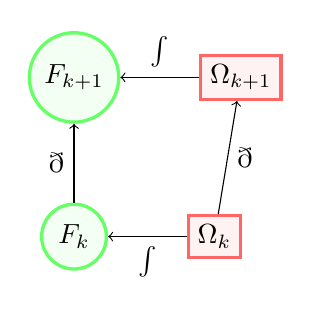
\begin{tikzpicture}
[roundnode/.style={circle, draw=green!60, fill=green!5, very thick, minimum size=7mm},
squarednode/.style={rectangle, draw=red!60, fill=red!5, very thick, minimum size=5mm},
]
\node[roundnode]	(f2) {$F_{k+1}$};
\node[roundnode]	(f1) [below=of f2]{$F_k$};
\node[squarednode]	(w2) [right=of f2] {$\Omega_{k+1}$};
\node[squarednode]	(w1) [right=of f1] {$\Omega_k$};

\draw[<-] (f2) -- (w2) node[midway, above] {$\int$};
\draw[<-] (f2) -- (f1) node[midway, left] {$\eth$};
\draw[<-] (f1) -- (w1) node[midway, below] {$\int$};
\draw[<-] (w2) -- (w1) node[midway, right] {$\eth$};
\end{tikzpicture}


\begin{defn}
	\textbf{Stoke's Theorem}: For (k-1)-form $\omega$ and k-surface $\sigma$, $\int_{\partial \sigma}\omega = \int_{\sigma}\eth\omega$. 
\end{defn}

NOTE: It seems that we don't even needs to worry about orientation as long as we're in coordinate free space. If possible, it would be cool to be able to not talk about orientation at all. It's just a choice of sign on both the direction of integration and the k-form. We can show that changing the sign of the integration necessitates also changing the sign of the k-form, thus making the orientation itself unnecessary (may not be needed). "suppose that you have a k-form, and you have chosen your coordinates, you can switch the order of integration and put a minus on the form, but then components of hte form change, so the form has different components dependign on orientation." "Or, we can say that there is some coordinate for which we go from a to be and others from b to a, components are thus the same, coordinates are different, but make up a class. It's just a different way to keep track of the sign." Components flip sign under a mirror, or flip, or whatever. 

NOTE: If we can stay coordinate free up until this point, maybe we can start talking about coordinates here in the coordinate transformation section
\section{Tensors and coordinate transformations}
Some quantities can undergo one-to-one transformations between coordinate systems. In general, such quantities are tensors. 


\begin{defn}
	A \textbf{tensor} is an object with a one-to-one relationship with objects between coordinate systems. 
\end{defn}

\begin{coro}
	A contravariant tensor of \textbf{rank 1} is a vector, which transforms as  $X'^a = \frac{\partial x'^a}{\partial x^b} X^b$.  
\end{coro}

\begin{coro}
	A covariant tensor of \textbf{rank 1} is a vector, which transforms as $X'_a = \frac{\partial x^b}{\partial x'^a} X_b$. 
\end{coro}

\begin{coro}
	A contravariant tensor of \textbf{rank 2} is a matrix $X^{ab}$ that transforms as $X'^{ab} = \frac{\partial x'^a}{\partial x^c} \frac{\partial x'^b}{\partial x^d} X^{cd}$. 
\end{coro}

\begin{coro}
	A contravariant tensor of \textbf{rank 0} is a quantity $X$ that transforms $X' = X$. Hence, a scalar. 
\end{coro}

- In general, objects associated with covariant tensors will have a lower index, and those associated with contravariant tensors will have an upper index. 












\chapter{Geometry and (States, Tensors, Forms)???}


\section{Symplectic geometry and state spaces}
We want to be able to represent our state configurations. Symplectic geometry arises when trying to describe their areas

\subsection{Symplectic form and areas}



\subsection{Metric tensor}
A more generalized inner product: feed in two vectors, and the outcome is a scalar representing the lengths of the vectors and the angle between them. 

\begin{defn}
	A \textbf{metric tensor g} is a function that takes two vectors and returns a real scalar. 
\end{defn}


\section{Riemannian geometry}
In order to give a mathematically rigorous definition of lengths of vectors and the angle between them, we use an inner product. Vector spaces with an inner product are Riemannian.

\begin{defn}
	Given two vectors $X^a,Y^a \in V$ and a metric tensor $g_{ab}$, the \textbf{inner product} $<X^a,Y^a> : V \times V \to \mathbb{R}$ is defined as $<X^a,Y^a> = g_{ab}X^aY^b$. 
\end{defn}

\begin{coro}
	The magnitude of $<u,v>$ is $|u||v|cos(\theta)$, where $\theta$ is the angle between u and v. 
\end{coro}

\begin{defn}
	If a vector space V contains an inner product, then V is \textbf{Riemannian}.
	\end{defn}



\subsection{Orthogonal basis}

\begin{defn}
	For contravariant vectors $X^a$ and $Y^a$, the two vectors are \textbf{orthogonal} if $<X^a,Y^b> = 0$. 
\end{defn}







\end{document}